\documentclass{article}\usepackage[]{graphicx}\usepackage[]{xcolor}
% maxwidth is the original width if it is less than linewidth
% otherwise use linewidth (to make sure the graphics do not exceed the margin)
\makeatletter
\def\maxwidth{ %
  \ifdim\Gin@nat@width>\linewidth
    \linewidth
  \else
    \Gin@nat@width
  \fi
}
\makeatother

\definecolor{fgcolor}{rgb}{0.345, 0.345, 0.345}
\newcommand{\hlnum}[1]{\textcolor[rgb]{0.686,0.059,0.569}{#1}}%
\newcommand{\hlsng}[1]{\textcolor[rgb]{0.192,0.494,0.8}{#1}}%
\newcommand{\hlcom}[1]{\textcolor[rgb]{0.678,0.584,0.686}{\textit{#1}}}%
\newcommand{\hlopt}[1]{\textcolor[rgb]{0,0,0}{#1}}%
\newcommand{\hldef}[1]{\textcolor[rgb]{0.345,0.345,0.345}{#1}}%
\newcommand{\hlkwa}[1]{\textcolor[rgb]{0.161,0.373,0.58}{\textbf{#1}}}%
\newcommand{\hlkwb}[1]{\textcolor[rgb]{0.69,0.353,0.396}{#1}}%
\newcommand{\hlkwc}[1]{\textcolor[rgb]{0.333,0.667,0.333}{#1}}%
\newcommand{\hlkwd}[1]{\textcolor[rgb]{0.737,0.353,0.396}{\textbf{#1}}}%
\let\hlipl\hlkwb

\usepackage{framed}
\makeatletter
\newenvironment{kframe}{%
 \def\at@end@of@kframe{}%
 \ifinner\ifhmode%
  \def\at@end@of@kframe{\end{minipage}}%
  \begin{minipage}{\columnwidth}%
 \fi\fi%
 \def\FrameCommand##1{\hskip\@totalleftmargin \hskip-\fboxsep
 \colorbox{shadecolor}{##1}\hskip-\fboxsep
     % There is no \\@totalrightmargin, so:
     \hskip-\linewidth \hskip-\@totalleftmargin \hskip\columnwidth}%
 \MakeFramed {\advance\hsize-\width
   \@totalleftmargin\z@ \linewidth\hsize
   \@setminipage}}%
 {\par\unskip\endMakeFramed%
 \at@end@of@kframe}
\makeatother

\definecolor{shadecolor}{rgb}{.97, .97, .97}
\definecolor{messagecolor}{rgb}{0, 0, 0}
\definecolor{warningcolor}{rgb}{1, 0, 1}
\definecolor{errorcolor}{rgb}{1, 0, 0}
\newenvironment{knitrout}{}{} % an empty environment to be redefined in TeX

\usepackage{alltt}
\usepackage[margin=1.0in]{geometry} % To set margins
\usepackage{amsmath}  % This allows me to use the align functionality.
                      % If you find yourself trying to replicate
                      % something you found online, ensure you're
                      % loading the necessary packages!
\usepackage{amsfonts} % Math font
\usepackage{fancyvrb}
\usepackage{hyperref} % For including hyperlinks
\usepackage[shortlabels]{enumitem}% For enumerated lists with labels specified
                                  % We had to run tlmgr_install("enumitem") in R
\usepackage{float}    % For telling R where to put a table/figure
\usepackage{natbib}        %For the bibliography
\bibliographystyle{apalike}%For the bibliography
\IfFileExists{upquote.sty}{\usepackage{upquote}}{}
\begin{document}

\begin{enumerate}
%%%%%%%%%%%%%%%%%%%%%%%%%%%%%%%%%%%%%%%%%%%%%%%%%%%%%%%%%%%%%%%%%%%%%%%%%%%%%%%%
%%%%%%%%%%%%%%%%%%%%%%%%%%%%%%%%%%%%%%%%%%%%%%%%%%%%%%%%%%%%%%%%%%%%%%%%%%%%%%%%
% QUESTION 1
%%%%%%%%%%%%%%%%%%%%%%%%%%%%%%%%%%%%%%%%%%%%%%%%%%%%%%%%%%%%%%%%%%%%%%%%%%%%%%%%
%%%%%%%%%%%%%%%%%%%%%%%%%%%%%%%%%%%%%%%%%%%%%%%%%%%%%%%%%%%%%%%%%%%%%%%%%%%%%%%%
\item Let's create some aRt! 
\begin{enumerate}
%%%%%%%%%%%%%%%%%%%%%%%%%%%%%%%%%%%%%%%%%%%%%%%%%%%%%%%%%%%%%%%%%%%%%%%%%%%%%%%%
% QUESTION 1a
%%%%%%%%%%%%%%%%%%%%%%%%%%%%%%%%%%%%%%%%%%%%%%%%%%%%%%%%%%%%%%%%%%%%%%%%%%%%%%%%
  \item Install the \texttt{aRtsy} package. Provide the code in an R chunk   that does 
  not run. You only need to install it one time.\\
\textbf{Solution: }
% Note that I have added eval=FALSE so that it won't run
% each time I compile
\begin{knitrout}\scriptsize
\definecolor{shadecolor}{rgb}{0.969, 0.969, 0.969}\color{fgcolor}\begin{kframe}
\begin{alltt}
\hlkwd{install.packages}\hldef{(}\hlsng{"aRtsy"}\hldef{)}
\end{alltt}
\end{kframe}
\end{knitrout}
%%%%%%%%%%%%%%%%%%%%%%%%%%%%%%%%%%%%%%%%%%%%%%%%%%%%%%%%%%%%%%%%%%%%%%%%%%%%%%%%
% QUESTION 1b
%%%%%%%%%%%%%%%%%%%%%%%%%%%%%%%%%%%%%%%%%%%%%%%%%%%%%%%%%%%%%%%%%%%%%%%%%%%%%%%%
  \item Load the \texttt{aRtsy} package. Provide the code in an R chunk that does run. 
  We need to load the library each time it is run.\\
\textbf{Solution:}
% Note here I have removed eval=FALSE so this code will run
\begin{knitrout}\scriptsize
\definecolor{shadecolor}{rgb}{0.969, 0.969, 0.969}\color{fgcolor}\begin{kframe}
\begin{alltt}
\hlkwd{library}\hldef{(aRtsy)}
\end{alltt}
\end{kframe}
\end{knitrout}
%%%%%%%%%%%%%%%%%%%%%%%%%%%%%%%%%%%%%%%%%%%%%%%%%%%%%%%%%%%%%%%%%%%%%%%%%%%%%%%%
% QUESTION 1c
%%%%%%%%%%%%%%%%%%%%%%%%%%%%%%%%%%%%%%%%%%%%%%%%%%%%%%%%%%%%%%%%%%%%%%%%%%%%%%%%
 \item Running \texttt{demo("aRtsy")} or \texttt{vignette("aRtsy")} don't return 
 any helpful demos or tutorials. However, if you run \texttt{help("aRtsy")} you 
 will find a link to a tutorial. Recreate the first figure they make using 
 \texttt{canvas\_collatz()}. Make sure to update the caption.\\
\textbf{Solution:}
\begin{knitrout}\scriptsize
\definecolor{shadecolor}{rgb}{0.969, 0.969, 0.969}\color{fgcolor}\begin{kframe}
\begin{alltt}
\hlkwd{help}\hldef{(}\hlsng{"aRtsy"}\hldef{)}
\hlkwd{set.seed}\hldef{(}\hlnum{1}\hldef{)}
\hlkwd{canvas_collatz}\hldef{(}\hlkwc{colors}\hldef{=}\hlkwd{colorPalette}\hldef{(}\hlsng{"tuscany3"}\hldef{))}
\end{alltt}
\end{kframe}
\end{knitrout}
%Code to insert a figure [H]ere
\begin{figure}[H]
\begin{center}
\begin{knitrout}
\definecolor{shadecolor}{rgb}{0.969, 0.969, 0.969}\color{fgcolor}
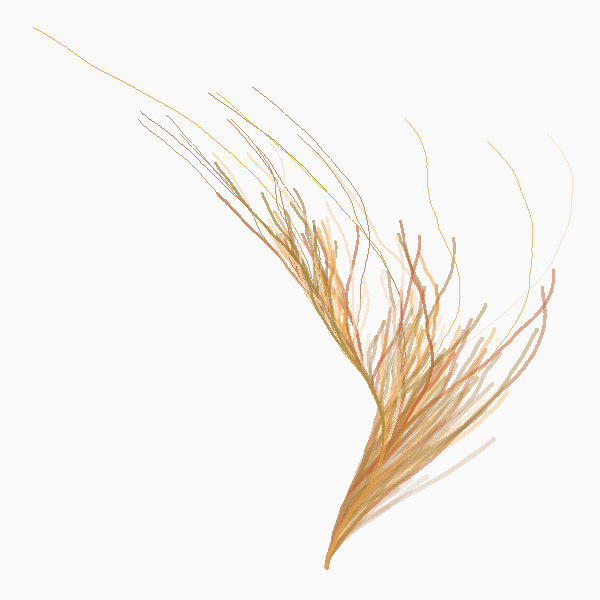
\includegraphics[width=\maxwidth]{figure/unnamed-chunk-3-1} 
\end{knitrout}
\caption{A collatz conjecture with a seed of 1}
\label{CollatzPlot1}
\end{center}
\end{figure}
%%%%%%%%%%%%%%%%%%%%%%%%%%%%%%%%%%%%%%%%%%%%%%%%%%%%%%%%%%%%%%%%%%%%%%%%%%%%%%%%
% QUESTION 1d
%%%%%%%%%%%%%%%%%%%%%%%%%%%%%%%%%%%%%%%%%%%%%%%%%%%%%%%%%%%%%%%%%%%%%%%%%%%%%%%%
  \item Change the randomization seed to 1313, which will change the random
  numbers generated to create the plot. Can you see the difference? Make sure to 
  update the caption.\\
\textbf{Solution:}
\begin{knitrout}\scriptsize
\definecolor{shadecolor}{rgb}{0.969, 0.969, 0.969}\color{fgcolor}\begin{kframe}
\begin{alltt}
\hlkwd{set.seed}\hldef{(}\hlnum{1313}\hldef{)}
\hlkwd{canvas_collatz}\hldef{(}\hlkwc{colors}\hldef{=}\hlkwd{colorPalette}\hldef{(}\hlsng{"tuscany3"}\hldef{))}
\end{alltt}
\end{kframe}
\end{knitrout}
%Code to insert a figure [H]ere
\begin{figure}[H]
\begin{center}
\begin{knitrout}
\definecolor{shadecolor}{rgb}{0.969, 0.969, 0.969}\color{fgcolor}
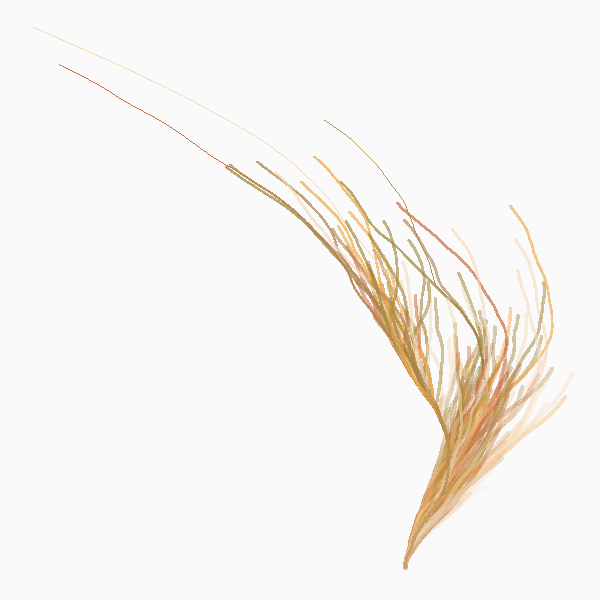
\includegraphics[width=\maxwidth]{figure/unnamed-chunk-4-1} 
\end{knitrout}
\caption{A collatz conjecture with a seed of 1313}
\label{CollatzPlot2}
\end{center}
\end{figure}
%%%%%%%%%%%%%%%%%%%%%%%%%%%%%%%%%%%%%%%%%%%%%%%%%%%%%%%%%%%%%%%%%%%%%%%%%%%%%%%%
% QUESTION 1e
%%%%%%%%%%%%%%%%%%%%%%%%%%%%%%%%%%%%%%%%%%%%%%%%%%%%%%%%%%%%%%%%%%%%%%%%%%%%%%%%
  \item Now, create a new Collatz conjecture plot by specifying the following 
  arguments. Note you will find the help file for the \texttt{canvas\_collatz()} 
  function to be rather helpful. Make sure to update the caption.
  \begin{itemize}
  \item Use the \texttt{vrolik4} color palette. Note you can find other by running 
  \texttt{?colorPalette} in the console.
  \item Make the background grey. Note a hexcode for grey is \texttt{\#dbdbdb}.
  \item Specify that there should be 72 strands.
  \item Specify the angle used for bending the sequence for odd numbers as -0.05.
  \item Specify the angle used for bending the sequence for even numbers as 0.0145 
  (note this is the default).
  \end{itemize}
\textbf{Solution:}
\begin{knitrout}\scriptsize
\definecolor{shadecolor}{rgb}{0.969, 0.969, 0.969}\color{fgcolor}\begin{kframe}
\begin{alltt}
\hlkwd{canvas_collatz}\hldef{(}\hlkwc{colors}\hldef{=}\hlkwd{colorPalette}\hldef{(}\hlsng{"vrolik4"}\hldef{),}
               \hlkwc{background} \hldef{=} \hlsng{"#dbdbdb"}\hldef{,}
               \hlkwc{n} \hldef{=} \hlnum{72}\hldef{,}
               \hlkwc{angle.even} \hldef{=} \hlnum{0.0145}\hldef{,}
               \hlkwc{angle.odd} \hldef{=} \hlopt{-}\hlnum{0.05}\hldef{)}
\end{alltt}
\end{kframe}
\end{knitrout}
%Code to insert a figure [H]ere
\begin{figure}[H]
\begin{center}
\begin{knitrout}
\definecolor{shadecolor}{rgb}{0.969, 0.969, 0.969}\color{fgcolor}
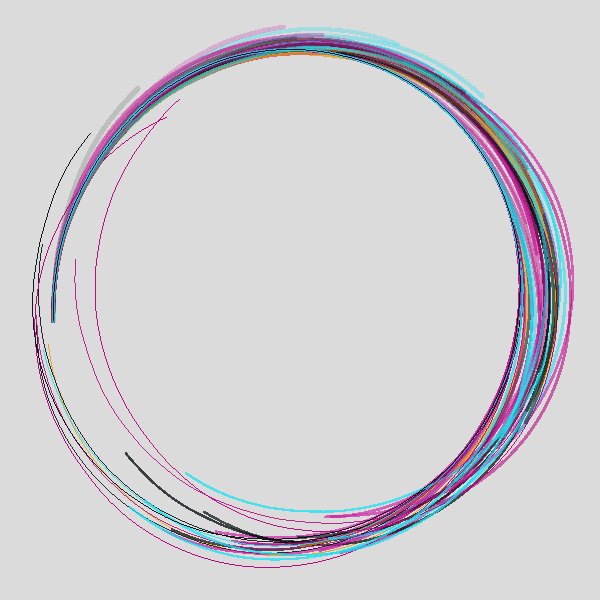
\includegraphics[width=\maxwidth]{figure/unnamed-chunk-5-1} 
\end{knitrout}
\caption{A collatz conjecture with a seed of 1313, 72 strands, and -0.05 angle for bending the odd number sequence.}
\label{CollatzPlot3}
\end{center}
\end{figure}
%%%%%%%%%%%%%%%%%%%%%%%%%%%%%%%%%%%%%%%%%%%%%%%%%%%%%%%%%%%%%%%%%%%%%%%%%%%%%%%%
% QUESTION 1f
%%%%%%%%%%%%%%%%%%%%%%%%%%%%%%%%%%%%%%%%%%%%%%%%%%%%%%%%%%%%%%%%%%%%%%%%%%%%%%%%
  \item Make another plot using the tutorial -- feel free to be creative here! 
  Note that I leave creating the R chunk and figure environment to you here. 
  Make sure that your code is well-formatted and your plot is appropriately scaled.\\
  \textbf{Solution:}
\begin{knitrout}\scriptsize
\definecolor{shadecolor}{rgb}{0.969, 0.969, 0.969}\color{fgcolor}\begin{kframe}
\begin{alltt}
\hlkwd{set.seed}\hldef{(}\hlnum{149}\hldef{)}
\hldef{colors} \hlkwb{<-} \hlkwd{list}\hldef{(}
  \hlkwd{c}\hldef{(}\hlsng{"darkseagreen"}\hldef{,} \hlsng{"darkslategray4"}\hldef{,}\hlsng{"deepskyblue4"}\hldef{,}\hlsng{"azure"}\hldef{),}
  \hlkwd{c}\hldef{(}\hlsng{"sienna3"}\hldef{,}\hlsng{"peru"}\hldef{,}\hlsng{'lightsalmon1'}\hldef{,}\hlsng{"ghostwhite"}\hldef{),}
  \hlkwd{c}\hldef{(}\hlsng{"orangered2"}\hldef{,}\hlsng{"orange"}\hldef{,} \hlsng{"tomato1"}\hldef{,}\hlsng{"coral"}\hldef{),}
  \hlkwd{c}\hldef{(}\hlsng{"ivory"}\hldef{,}\hlsng{"azure"}\hldef{,}\hlsng{"mintcream"}\hldef{,}\hlsng{"grey"}\hldef{,}\hlsng{"grey100"}\hldef{,}\hlsng{"lightgrey"}\hldef{)}
\hldef{)}

\hlkwd{canvas_planet}\hldef{(colors,}
              \hlkwc{starprob}\hldef{=}\hlnum{0.005}\hldef{,}
              \hlkwc{radius} \hldef{=} \hlkwd{c}\hldef{(}\hlnum{300}\hldef{,} \hlnum{200}\hldef{,} \hlnum{1500}\hldef{,} \hlnum{100}\hldef{),}
              \hlkwc{center.x}\hldef{=} \hlkwd{c}\hldef{(}\hlnum{750}\hldef{,} \hlnum{1900}\hldef{,} \hlopt{-}\hlnum{1100}\hldef{,} \hlnum{1200}\hldef{),}
              \hlkwc{center.y}\hldef{=} \hlkwd{c}\hldef{(}\hlnum{700}\hldef{,} \hlnum{700}\hldef{,} \hlnum{1000}\hldef{,} \hlnum{700}\hldef{),}
              \hlkwc{light.right} \hldef{=} \hlnum{FALSE}\hldef{,}
              \hlkwc{resolution} \hldef{=} \hlnum{2000}
              \hldef{)}
\end{alltt}
\end{kframe}
\end{knitrout}
%Code to insert a figure [H]ere
\begin{figure}[H]
\begin{center}
\begin{knitrout}
\definecolor{shadecolor}{rgb}{0.969, 0.969, 0.969}\color{fgcolor}
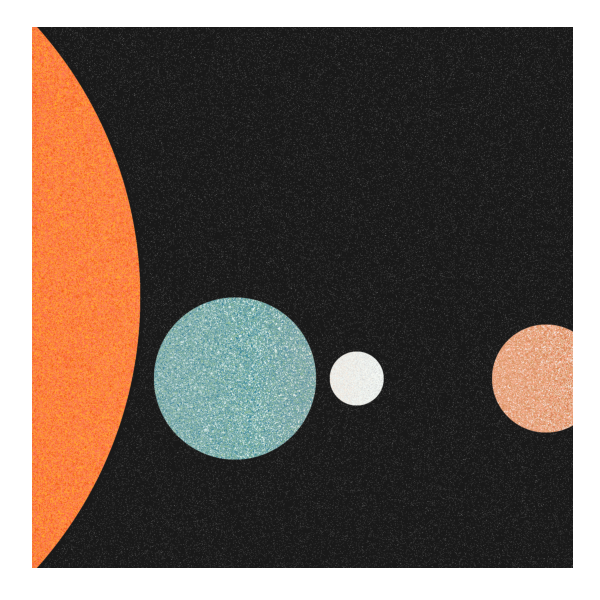
\includegraphics[width=\maxwidth]{figure/unnamed-chunk-6-1} 
\end{knitrout}
\caption{A planet plot of an Earth-like planet, a moon, and a Mars-like planet.}
\label{PlanetPlot1}
\end{center}
\end{figure}
%%%%%%%%%%%%%%%%%%%%%%%%%%%%%%%%%%%%%%%%%%%%%%%%%%%%%%%%%%%%%%%%%%%%%%%%%%%%%%%%
% QUESTION 1g
%%%%%%%%%%%%%%%%%%%%%%%%%%%%%%%%%%%%%%%%%%%%%%%%%%%%%%%%%%%%%%%%%%%%%%%%%%%%%%%%
  \item Use \texttt{citation()} to get the BiBTeX citation for the \texttt{aRtsy}
  package and use \verb|\citep{}| to add a parenthetical citation to the end of
  the sentence below.
\textbf{Solution:} We created the generative art in Question 1 using the \texttt{aRtsy}
package for \texttt{R} \citep{aRtsy}.
\end{enumerate}

\newpage

%%%%%%%%%%%%%%%%%%%%%%%%%%%%%%%%%%%%%%%%%%%%%%%%%%%%%%%%%%%%%%%%%%%%%%%%%%%%%%%%
%%%%%%%%%%%%%%%%%%%%%%%%%%%%%%%%%%%%%%%%%%%%%%%%%%%%%%%%%%%%%%%%%%%%%%%%%%%%%%%%
% QUESTION 2
%%%%%%%%%%%%%%%%%%%%%%%%%%%%%%%%%%%%%%%%%%%%%%%%%%%%%%%%%%%%%%%%%%%%%%%%%%%%%%%%
%%%%%%%%%%%%%%%%%%%%%%%%%%%%%%%%%%%%%%%%%%%%%%%%%%%%%%%%%%%%%%%%%%%%%%%%%%%%%%%%
\item Suppose we wanted to solve $2^{x+1} +2^{x-1} = 40$ for $x$. While this is a pretty straightforward algebra problem, it's useful for demonstrating the use of objects in R. 
  \begin{enumerate}
  %%%%%%%%%%%%%%%%%%%%%%%%%%%%%%%%%%%%%%%%%%%%%%%%%%%%%%%%%%%%%%%%%%%%%%%%%%%%%%%%
  % QUESTION 2a
  %%%%%%%%%%%%%%%%%%%%%%%%%%%%%%%%%%%%%%%%%%%%%%%%%%%%%%%%%%%%%%%%%%%%%%%%%%%%%%%%
  \item Create a numeric vector containing the integers from 0 to 10 inclusive. Hint -- the solution to this problem is one of these values.\\
\textbf{Solution:}
\begin{knitrout}\scriptsize
\definecolor{shadecolor}{rgb}{0.969, 0.969, 0.969}\color{fgcolor}\begin{kframe}
\begin{alltt}
\hldef{vector1} \hlkwb{=} \hlkwd{c}\hldef{(}\hlnum{0}\hlopt{:}\hlnum{10}\hldef{)} \hlcom{#creates a vector of the integers from 0 to 10}
\end{alltt}
\end{kframe}
\end{knitrout}
  %%%%%%%%%%%%%%%%%%%%%%%%%%%%%%%%%%%%%%%%%%%%%%%%%%%%%%%%%%%%%%%%%%%%%%%%%%%%%%%%
  % QUESTION 2b
  %%%%%%%%%%%%%%%%%%%%%%%%%%%%%%%%%%%%%%%%%%%%%%%%%%%%%%%%%%%%%%%%%%%%%%%%%%%%%%%%
  \item Complete the algebra to compute $2^{x+1} +2^{x-1}$ for each value in the numerical vector created in step 1. Make sure to save the result to a new numeric vector.\\
\textbf{Solution:}
\begin{knitrout}\scriptsize
\definecolor{shadecolor}{rgb}{0.969, 0.969, 0.969}\color{fgcolor}\begin{kframe}
\begin{alltt}
\hldef{completed_algebra} \hlkwb{<-} \hlkwd{c}\hldef{()}
\hlkwa{for} \hldef{(x} \hlkwa{in} \hldef{vector1)\{}
  \hldef{equation1} \hlkwb{<-} \hlnum{2}\hlopt{^}\hldef{(x}\hlopt{+}\hlnum{1}\hldef{)} \hlopt{+} \hlnum{2}\hlopt{^}\hldef{(x}\hlopt{-}\hlnum{1}\hldef{)} \hlcom{#left side of the equation; = 40}
  \hldef{completed_algebra} \hlkwb{<-} \hlkwd{append}\hldef{(completed_algebra, equation1)}
\hldef{\}}
\end{alltt}
\end{kframe}
\end{knitrout}
  %%%%%%%%%%%%%%%%%%%%%%%%%%%%%%%%%%%%%%%%%%%%%%%%%%%%%%%%%%%%%%%%%%%%%%%%%%%%%%%%
  % QUESTION 2c
  %%%%%%%%%%%%%%%%%%%%%%%%%%%%%%%%%%%%%%%%%%%%%%%%%%%%%%%%%%%%%%%%%%%%%%%%%%%%%%%%
  \item Use the which() function to ask which result is 40.\\
\textbf{Solution:}
\begin{knitrout}\scriptsize
\definecolor{shadecolor}{rgb}{0.969, 0.969, 0.969}\color{fgcolor}\begin{kframe}
\begin{alltt}
\hldef{answerQ2} \hlkwb{<-} \hlkwd{which}\hldef{(completed_algebra} \hlopt{==} \hlnum{40}\hldef{)}
\end{alltt}
\end{kframe}
\end{knitrout}
  %%%%%%%%%%%%%%%%%%%%%%%%%%%%%%%%%%%%%%%%%%%%%%%%%%%%%%%%%%%%%%%%%%%%%%%%%%%%%%%%
  % QUESTION 2d
  %%%%%%%%%%%%%%%%%%%%%%%%%%%%%%%%%%%%%%%%%%%%%%%%%%%%%%%%%%%%%%%%%%%%%%%%%%%%%%%%
  \item What is the solution? That is, what value of x yields $2^{x+1} +2^{x-1} = 40$?\\
\textbf{Solution:}

$x = 4$
  %%%%%%%%%%%%%%%%%%%%%%%%%%%%%%%%%%%%%%%%%%%%%%%%%%%%%%%%%%%%%%%%%%%%%%%%%%%%%%%%
  % QUESTION 2e
  %%%%%%%%%%%%%%%%%%%%%%%%%%%%%%%%%%%%%%%%%%%%%%%%%%%%%%%%%%%%%%%%%%%%%%%%%%%%%%%%
  \item Explain why this approach wouldn't work for something like $3^{x+2} + 5 (3^x) = 84$ where the solution is $x \approx 1.6309$.\\
\textbf{Solution:}
This approach assumed that x is an integer between 0 and 10. We began and based all of our work off of that when we created the vector from 0-10 and tried every value in it, to see which was correct. This is more akin to "guess and check" than actual algebra, which is needed in more complicated problems.
\end{enumerate}
\end{enumerate}

\end{document}
